
% ==========================================================
\section{Evaluation Plan}
% ==========================================================
\arman{Sectoins starting from here should be about 2 pages}

% ==========================================================
\section{Broader Impacts}
% ==========================================================

\textbf{Securing real-world infrastructure.}
This project directly targets the classes of devices responsible for the field-deployed compromises surveyed in the Overview: automotive infotainment ECUs~\cite{perfektblue2025}, industrial water and wastewater controllers~\cite{cisa2023unitronics}, and the embedded TCP/IP stacks used across healthcare, industrial, and transportation systems~\cite{cisa2020ripple20}. By making embedded trust verifiable at construction, runtime, and recovery, \sys directly reduces the attack surface and remediation cost for the operators and manufacturers of exactly this class of field-deployed, unattended devices.

\textbf{Influencing standards and industry practice.}
Federal guidance including NIST's IoT Core Baseline~\cite{nist2022ir8425}, the FDA's premarket cybersecurity guidance for medical devices~\cite{fda2023cybersecurity}, and CISA's Secure-by-Design principles~\cite{cisa2023sbd} all call for built-in, continuously verifiable device trustworthiness, but none prescribes concrete mechanisms. \sys's composition attestation, runtime evidence, and evidence-guided recovery mechanisms provide candidate building blocks that manufacturers and standards bodies can adopt to meet these emerging requirements.

\textbf{Broadening participation.}
UTEP is an R1 research university and a Hispanic-Serving Institution, and Hispanic students remain severely underrepresented in cybersecurity and hardware security research nationally. By funding and training graduate and undergraduate students at UTEP in embedded and hardware security, this project will broaden participation of Hispanic and other underrepresented students in a subfield with few existing training pipelines.

\begin{wrapfigure}{r}{0.4\textwidth}
	\centering
	\vspace{-8pt}
	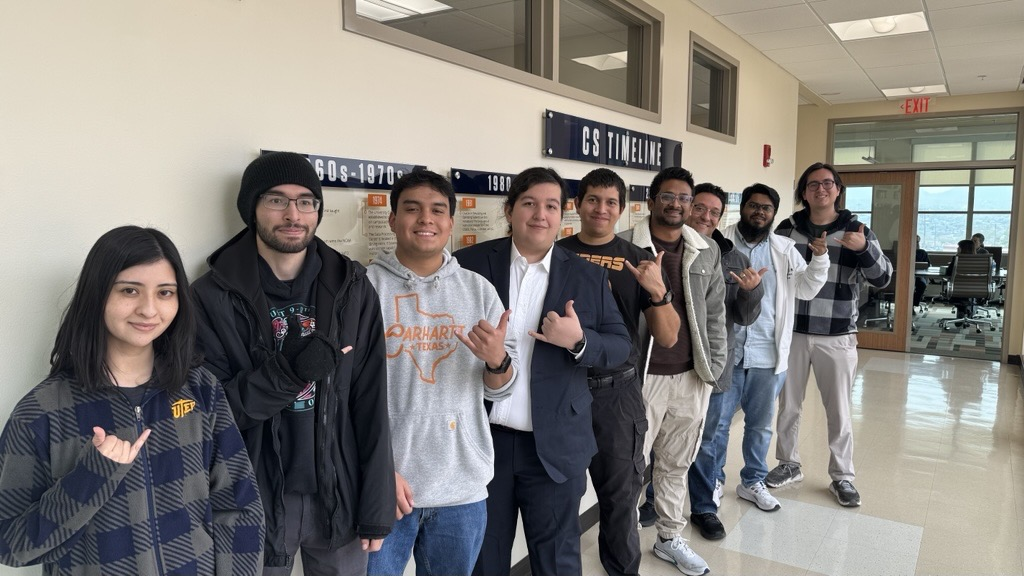
\includegraphics[width=0.38\textwidth]{figs/01.png}\\[4pt]
	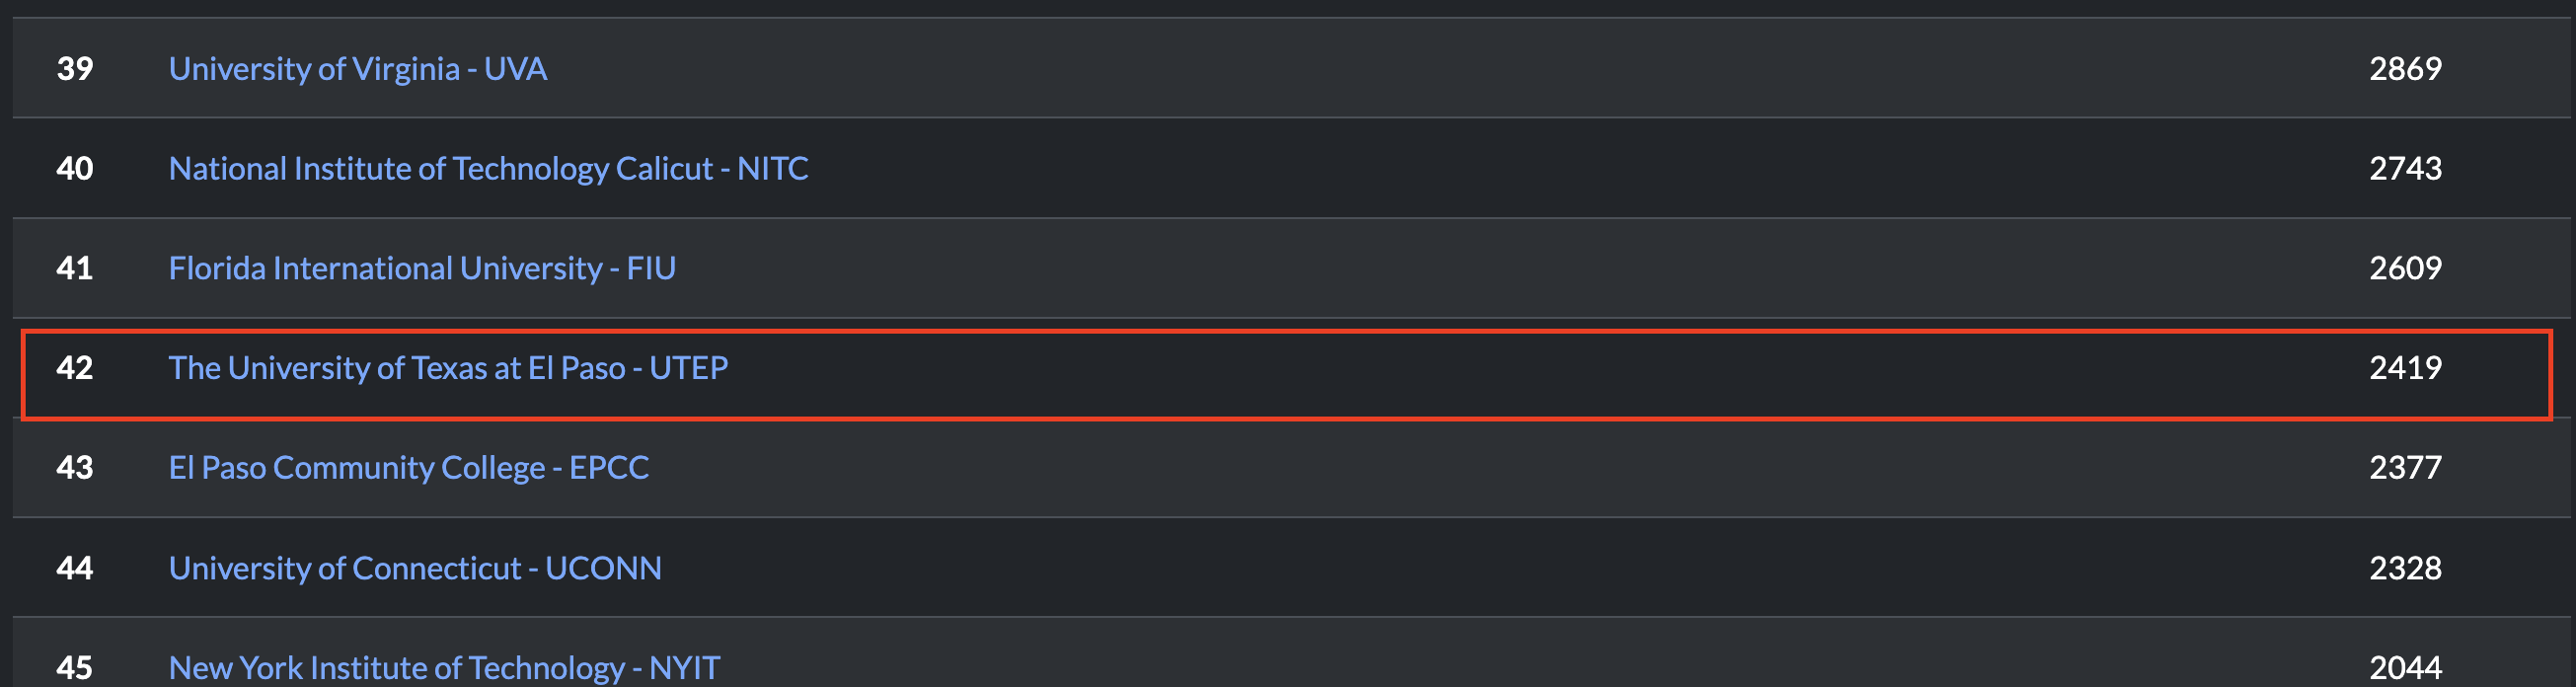
\includegraphics[width=0.38\textwidth]{figs/02_crop.png}
	\caption{Team UTEP at the 2026 MITRE eCTF (top) and the team's ranking on the competition scoreboard (bottom).}
	\label{fig:ectf}
	\vspace{-8pt}
\end{wrapfigure}
\textbf{Education and workforce development.}
Building on the PI's seven years of MITRE eCTF experience as team member, captain, and now faculty advisor, the project will continue to mentor a student team through the competition's Cortex-M-based embedded security challenges (Figure~\ref{fig:ectf}), using project outcomes as training material and giving students hands-on experience directly transferable to industry and research careers.

\textbf{Embedded systems security curricular development.}
The PI currently teaches CS 4390/5390 \textit{System Security: Attack and Defense for Binaries} at UTEP, which covers offensive techniques (buffer overflow, ROP, shellcoding) and defensive techniques (stack canaries, shadow stacks, ASLR, control-flow integrity) through hands-on labs and in-class CTF competitions. Outcomes from this project, including control-flow attestation and hardware-assisted compartmentalization, extend this curriculum from software-only mitigations to hardware-rooted, verifiable defenses, and lessons learned from the PI's MITRE eCTF advising will directly inform new embedded-focused lab assignments and CTF challenges.

\textbf{Open-source artifacts.}
The \byotee and \enola prototypes underlying Thrusts~1 and~2 are already open-sourced, and the new trusted-domain, attestation, and compartmentalization toolchains developed in this project will likewise be released as open-source under a permissive license, consistent with the project's data management plan, lowering the barrier for other researchers, educators, and practitioners to reproduce, extend, and adopt these results.

% ==========================================================
\section{Proposed Project Timeline}
% ==========================================================
\begin{wrapfigure}{r}{0.5\textwidth}
	\centering
	\vspace{-8pt}
	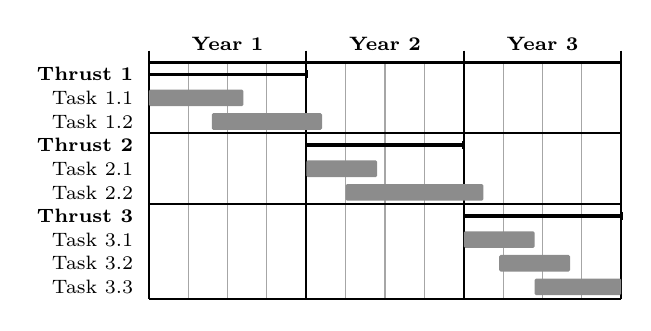
\begin{tikzpicture}[x=0.5cm, y=-0.3cm, font=\scriptsize]
		% --- header: year labels ---
		\node[font=\bfseries\scriptsize] at (2,-0.8)  {Year 1};
		\node[font=\bfseries\scriptsize] at (6,-0.8)  {Year 2};
		\node[font=\bfseries\scriptsize] at (10,-0.8) {Year 3};

		% --- thick vertical year-boundary / outer border lines (span header to bottom) ---
		\foreach \x in {0,4,8,12} {
			\draw[thick] (\x,-0.5) -- (\x,10);
		}
		% --- thin quarter gridlines (grid area only) ---
		\foreach \x in {1,2,3,5,6,7,9,10,11} {
			\draw[black!35, thin] (\x,0) -- (\x,10);
		}
		% --- thick horizontal borders: top, between thrust groups, bottom ---
		\foreach \y in {0,3,6,10} {
			\draw[thick] (0,\y) -- (12,\y);
		}

		% --- row labels ---
		\node[anchor=east, font=\bfseries\scriptsize] at (-0.15,0.5) {Thrust 1};
		\node[anchor=east, font=\scriptsize] at (-0.15,1.5) {Task 1.1};
		\node[anchor=east, font=\scriptsize] at (-0.15,2.5) {Task 1.2};

		\node[anchor=east, font=\bfseries\scriptsize] at (-0.15,3.5) {Thrust 2};
		\node[anchor=east, font=\scriptsize] at (-0.15,4.5) {Task 2.1};
		\node[anchor=east, font=\scriptsize] at (-0.15,5.5) {Task 2.2};

		\node[anchor=east, font=\bfseries\scriptsize] at (-0.15,6.5) {Thrust 3};
		\node[anchor=east, font=\scriptsize] at (-0.15,7.5) {Task 3.1};
		\node[anchor=east, font=\scriptsize] at (-0.15,8.5) {Task 3.2};
		\node[anchor=east, font=\scriptsize] at (-0.15,9.5) {Task 3.3};

		% --- thrust duration bars (bold, with small end tick) ---
		\foreach \xa/\xb/\yy in {0/4/0.5, 4/8/3.5, 8/12/6.5} {
			\draw[very thick] (\xa,\yy) -- (\xb,\yy);
			\draw[very thick] (\xb,{\yy-0.16}) -- (\xb,{\yy+0.16});
		}

		% --- task bars (gray, staggered, last task of T1/T2 overlaps into next year) ---
		\foreach \xa/\xb/\rr in {0/2.4/1, 1.6/4.4/2, 4/5.8/4, 5.0/8.5/5, 8/9.8/7, 8.9/10.7/8, 9.8/12/9} {
			\draw[fill=black!45, draw=none, rounded corners=0.5pt] (\xa,{\rr+0.15}) rectangle (\xb,{\rr+0.85});
		}
	\end{tikzpicture}
	\caption{Proposed project timeline.}
	\label{fig:timeline}
	\vspace{-8pt}
\end{wrapfigure}
Figure~\ref{fig:timeline} shows the proposed three-year schedule. The three thrusts are sequenced so that each stage's output grounds the next: Thrust~1 (Year~1) establishes application-specific trusted domains on FPGA SoC and ARM~CCA platforms; Thrust~2 (Year~2) builds scalable runtime attestation on top of the resulting trust boundary; and Thrust~3 (Year~3) develops evidence-guided compartmentalization and recovery using the runtime evidence from Thrust~2. Tasks within each thrust are staggered, and the final task of Thrusts~1 and~2 overlaps into the following year to allow early integration with the next thrust's prototypes.

% ==========================================================
\section{Results from Prior NSF Support}
% ==========================================================
The PI has no prior or current NSF support to report in last five years.